\section{Theorie}
\label{sec:Theorie}
Die Modulation und Demodulation
elektrischer Schwingungen wird
zur Informationsübertragung genutzt.
Dabei wird mit Hilfe der Modulation
(siehe Kapitel \ref{subsec:modulationsverfahren})
Amplitude, Frequenz oder auch die Phase
der Welle dem Nachrichtensignal entsprechend
verändert.
Um der modulierten Welle die Information
wieder zu entnehmen werden am Empfangsort
Demodulationsverfahren verwendet.

\subsection{Modulationsverfahren}
\label{subsec:modulationsverfahren}
Es existierten in der Hochfrequenztechnik einige
Verfahren zur Modulation, die unterschiedlichen
Anforderungen erfüllen. Grob können diese
jedoch in 2 Verfahren unterteilt
werden, einmal die Amplitudenmodulation \ref{subsubsec:amplitudenmodulation}
und die Frequenzmodulation \ref{subsubsec:frequenzmodulation}.

\subsubsection{Amplitudenmodulation}
\label{subsubsec:amplitudenmodulation}
Die Amplitudenmodulation kennzeichnet sich
dadurch, dass sich dabei die Signalamplitude
des Trägers $U_{\text{T}}(t)$ periodisch verändert.
Die Veränderung der Amplitude ist dabei gegeben
durch die Frequenz der Modulationsschwingung
$U_{\text{M}}(t)$.
Ausgehend von den Darstellungen der Signale
\begin{align}
U_{\text{T}} &= \hat{U}_{\text{T}} \, \cos \omega_{\text{T}} \, t \\
U_{\text{M}} &= \hat{U}_{\text{M}} \, \cos \omega_{\text{M}} \, t
\end{align}
mit den jeweiligen Kreisfrequenzen $\omega_{\text{T}}$ und $\omega_{\text{M}}$,
ergibt sich für das aus der Amplitudenmodulation resultierende Signal
\begin{align}
\label{eqn:1}
U_{3}(t) = \hat{U}_{\text{T}} \, \left( 1 + m \, \cos \omega_{\text{M}} t \right) \, .
\end{align}

Dabei ist $m$, der zu $U_{\text{M}}Q$ proportionale, Modulationsgrad.
Der zugehörige Proportionalitätsfaktor heißt $\gamma$.
Es gilt $0 \leq m \leq 1$.
In Abbildung \ref{fig:amplitudenmodulation_1} ist das Signal aus Gleichung
\eqref{eqn:1} dargestellt.
Dieses lässt sich so Umformen, dass die auftretenden Frequenzen direkt
ablesbar sind
\begin{align}
\label{eqn:2}
U_{\text{T}} &= \hat{U}_{\text{T}} \, \left( \cos \omega_{\text{T}} t \, + \, \frac{m}{2} \cos t\left( \omega_{\text{T}} + \omega_{\text{T}} \right) \, + \, \frac{m}{2} m \cos t \left( \omega_{\text{M}} - \omega_{\text{T}} \right)\right) \, .
\end{align}
Im Gegensatz zu den beiden Frequenzen $\omega_{\text{T}} + \omega_{\text{M}}$ und $\omega_{\text{T}} - \omega_{\text{M}}$, tritt die Frequenz $\omega_{\text{T}}$
unabhängig von $U_{\text{M}}$ auf und spielt somit
für die Informationsübertragung keine Rolle. Daher soll $\omega_{\text{T}}$
aus Gründen der Energieeffizienz herausgefiltert werden.
Aus den beiden übrigen Frequenzlinien werden, wenn das Modulationssignal
aus mehreren Frequenzen zusammengesetzt ist, Frequenzbänder.
Diese tragen jeweils dieselbe Information, sodass eines der beiden ohne
Informationsverlust unterdrückt werden kann(\textit{Einseitenbandmodulation}).\\ \\

Probleme der Amplitudenmodulation stellen die geringe Toleranz gegenüber
Störungen, sowie die geringe Verzerrungsfreiheit dar.

\begin{figure}
\centering
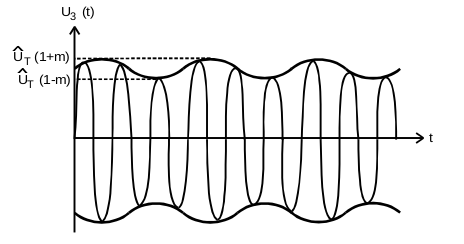
\includegraphics[width=0.7\textwidth]{figures/amplitudenmodulation.PNG}
\caption{Zeitlicher Verlauf einer amplitudenmodulierten Schwingung.\cite{sample}}
\label{fig:amplitudenmodulation_1}
\end{figure}

\subsubsection{Frequenzmodulation}
\label{subsubsec:frequenzmodulation}
Bei der Frequenzmodulation wird die
momentane Schwingungsfrequenz
abhängig
von dem Modulationssignal und die
Amplitude der Schwingung bleibt konstant.
Die Schwingung nimmt dann folgende Form an
\begin{align}
U(t) = \hat{U} \sin\left(\omega_{\text{T}} t + m\frac{\omega_{\text{T}}}{\omega_{\text{M}}} \cos\omega_{\text{M}}t \right),\label{eqn:3}
\intertext{mit der Momentanfrequenz}
f(t)=\frac{\omega_{\text{T}}}{2\pi} \left(1-m\sin\omega_{\text{M}}t\right)\label{eqn:f}
\end{align}
wobei $m$ dem Modulationsgrad
entspricht.
Die Variationsbreite
der Schwingungsfrequenz
wird Frequenzhub genannt und entspricht
$m \, \sfrac{\omega_{\text{T}}}{2\pi}$.
Die Abbildung \ref{fig:frequenzmodulation}
enthält einen beispielhaften Verlauf
einer Frequenzmodulation.

\begin{figure}
\centering
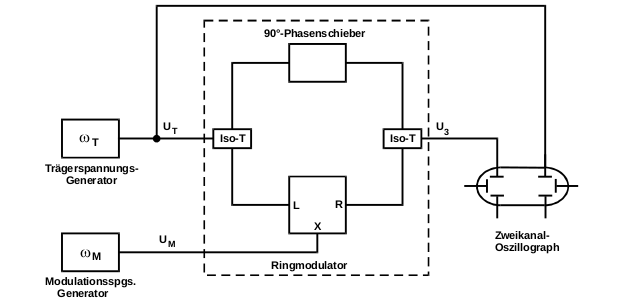
\includegraphics[width=0.7\textwidth]{figures/frequenzmodulator.PNG}
\caption{Zeitlicher Verlauf einer frequenzmodulierten Schwingung.}
\label{fig:frequenzmodulation}
\end{figure}

Wird nur der Fall eines
niedrigens Frequenzhubes
betrachtet, kann die Gleichung
\begin{align*}
m \, \frac{\omega_{\text{T}}}{\omega_{\text{M}}} \ll 1
\end{align*}
\eqref{eqn:3} durch Nährungen
in die Form
\begin{align}
\hat{U}(t)=\hat{U}\left(\sin \omega t + \frac12 m\frac{\omega_{\text{T}}}{\omega_{\text{M}}}\cos t(\omega_{\text{T}}+\omega_{\text{M}})
+ \frac12 m\frac{\omega_{\text{T}}}{\omega_{\text{M}}}\cos t(\omega_{\text{T}}-\omega_{\text{M}}) \right)
\end{align}
gebracht werden.
Daraus kann entnommen werden, dass
bei schwach frequenzmodulierten Schwingungen
ebenso wie bei amplitudenmodulierten
drei Teilschwingungen mit den Frequenzen $\omega_{\text{T}},\omega_{\text{T}}+\omega_{\text{M}}$
und $\omega_{\text{T}}-\omega_{\text{M}}$ existieren.
Dabei sind die Seitenlinien $\omega_{\text{T}}\pm\omega_{\text{M}}$
um $\sfrac{\pi}{2}$ zur Trägerschwingung verschoben.

\FloatBarrier

\subsection{Schaltungen}
\label{subsec:schaltungen}
Um die im Kapitel \ref{subsec:modulationsverfahren}
beschriebenen Modulationsverfahren so wie Demodulationsverfahren zu realisiert, werden
bestimmte elektronische Schaltungen
benötigt auf die im Folgenden näher eingegangen werden soll.

\subsubsection{Modulationsschaltungen}
\label{subsubsec:modulationsschaltungen}
\paragraph{Amplitudenmodulation}
\mbox{}\\
Für die Amplitudenmodulation
wird ein Gerät benötigt, das ein
Produkt zweier Spannungen bildet.
Bauteile mit einer nichtlinearen Kennlinie
erfüllen diese Bedingung wie zum Beispiel eine
Diode.
Somit lässt sich eine Modulatorschaltung
wie in Abbildung \ref{fig:diode}
mit einer Diode realisieren.
\begin{figure}
\centering
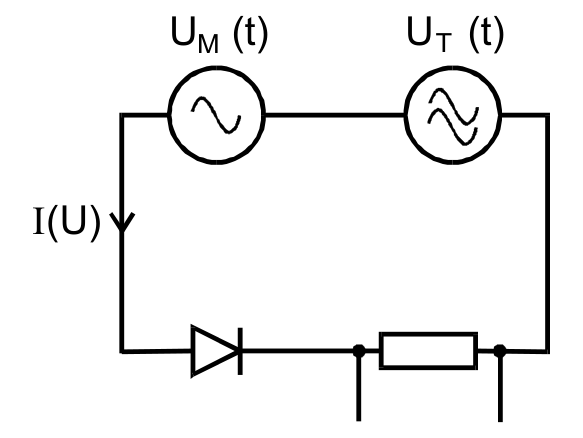
\includegraphics[width=0.5\textwidth]{figures/diode.PNG}
\caption{Primitive Modulatorschaltung mit Diode.\cite{sample}}
\label{fig:diode}
\end{figure}
Über die Reihenentwicklung der
Diodenkennlinie ergibt der gewünschte
Term $U_{\text{T}}U_{\text{M}}$ jedoch
treten dabei weitere störende Terme
auf wie z.B. $U_{\text{M}}, U_{\text{M}}^2$ und $U_{\text{T}}^2$.
Da diese normalerweise Frequenzen
besitzen, die weit außerhalb des
Frequenzbandes $[\omega_{\text{T}}-\omega_{\text{M}},\omega_{\text{T}}+\omega_{\text{M}}]$ liegen,
können diese mit Hilfe eines Bandfilters unterdrückt werden.
Eine bessere Methode zur Amplitudenmodulation
stellt ein
\textit{Ringmodulator} dar, da dieser
erst gar nicht die unerwünschten Komponenten
erzeugt.
Ein \textit{Ringmodulator} besteht aus
4 zu einem Ring geschaltenten Dioden,
wie in Abbildung
\ref{fig:5} dargestellt.

\begin{figure}
\centering
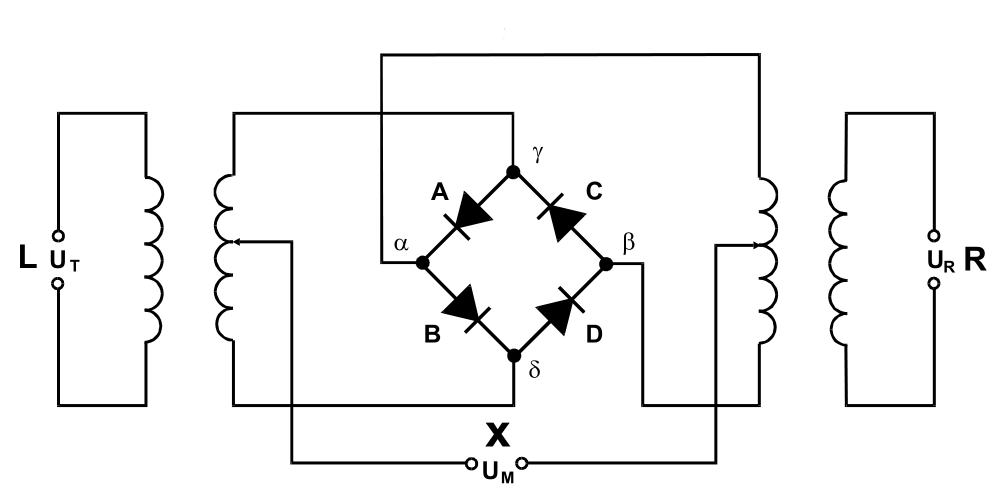
\includegraphics[width=0.7\textwidth]{figures/ringmodulator.PNG}
\caption{Schaltbild eines Ringmodulators.\cite{sample}}
\label{fig:5}
\end{figure}

Für übereinstimmende elektrische Eigenschaften
der 4 Dioden und einer Modulationsspannung $U_{\text{M}}=0$
tritt zwischen den Punkten $\alpha$ und $\beta$
keine Spannung auf. Für eine Modulationsspannung
$U_{\text{M}}\neq0$ folgt somit eine
Spannung $U_{\text{R}}$ am Ausgang, die die
Geichung
\begin{align}
  U_{\text{R}}(t) &= \gamma U_{\text{M}}(t)U_{\text{T}}(t)
\intertext{erfüllt. Somit ergibt sich durch Einsetzten
der Modulation- und Trägerspannung}
  U_{\text{T}}(t) &=\hat{U}_{\text{T}}\cos\omega_{\text{T}}t\\
  U_{\text{M}}(t) &= \hat{U}_{\text{M}}\cos(\omega_{\text{M}}t+\phi)
\intertext{eine Ausgangsspannung }
U_{\text{R}}(t) &=\gamma \hat{U}_{\text{T}} \hat{U}_{\text{M}}\frac{1}{2}\cos\left((\omega_{\text{T}}+\omega_{\text{M}})t+\phi\right) + \gamma \hat{U}_{\text{T}} \hat{U}_{\text{M}}\frac{1}{2}\cos\left((\omega_{\text{T}}-\omega_{\text{M}})t-\phi\right)
\end{align}
ohne Trägerabstrahlung.


\paragraph{Frequenzmodulation}
\mbox{}\\
Für eine Frequenzmodulation, die einen geringen Frequenzhub besitzt,
kann die in Abbildung \ref{fig:6} dargestellte
Schaltung verwendet werden.
Der \textit{Ringmodulator} erzeugt die Frequenzen der beiden Seitenbänder.
Zu diesem Signal wird zusätzlich die um $\SI{90}{\degree}$ phasenverschobene
Spannung der Trägerschwingung addiert.
% Dabei wird der Phasen-Shift
% mit einem Laufzeitkabel generiert.

\begin{figure}
\centering
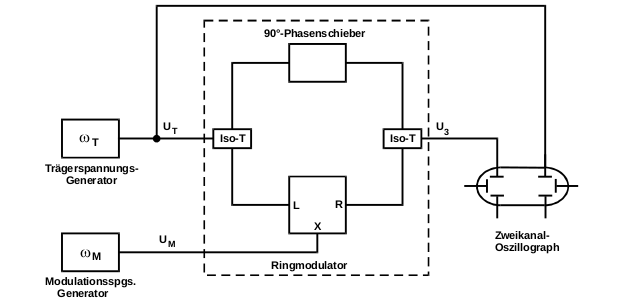
\includegraphics[width=0.7\textwidth]{figures/frequenzmodulator.PNG}
\caption{Schaltbild eines Ringmodulators für frequenzmodulierte Signale.\cite{sample}}
\label{fig:6}
\end{figure}

\subsubsection{Demodulationsschaltungen}
\label{subsubsec:demodulationschaltungen}
\paragraph{Demodulationsschaltung für amplitudenmodulierte Signale}
\mbox{}\\
Um aus einem modulierten Signal wieder die gewünschte Information zu erhalten,
müssen Träger- und Modulationssignal voneinander getrennt werden.
Dies geschieht mit einem Demodulator.\\
Als Demodulator kann der in Kapitel \ref{subsubsec:modulationsschaltungen}
vorgestellte \textit{Ringmodulator} genutzt werden.
Dazu wird auf den Eingang \textbf{R} das modulierte Signal und
auf \textbf{L} das Trägersignal, so erzeugt die Schaltung
ein Signal mit den Frequenzen
$\omega_{\text{M}}$, $2\omega_{\text{T}} - \omega_{\text{M}}$
und $2\omega_{\text{T}} + \omega_{\text{M}}$.
Um aus diesem Signal auschließlich $\omega_{\text{M}}$ zu gewinnen,
werden die beiden übrigen Frequenzen, die üblicherweise deutlich größer sind,
mit Hilfe eines Tiefpasses herausgefiltert.\\
In Abbildung \ref{fig:7} ist eine solche Schaltung gezeigt,
bei der der Ringmodulator zur Demodulation genutzt wird. Allerdings
birgt diese Methode den Nachteil, dass die für die Demodulation genutze
Spannung keine Phasenverschiebung gegenüber der Trägerfrequenz des
modulierten Signals besitzt.
Um dies zu umgehen, kann eine in Abbildung \ref{fig:8} gezeigte
Schaltung verwendet werden. In dieser wird eine Gleichrichter-Diode verwendet,
die dafür sorgt, dass keine negativen Spannungen mehr auftreten.
Es ergibt sich dann der in Abbildung \ref{fig:gleichgerichtet}
skizzierte Spannungsverlauf.




\begin{figure}
\centering
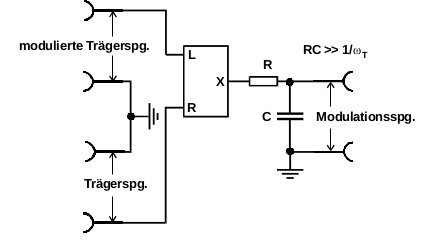
\includegraphics[width=0.7\textwidth]{figures/demodulator.PNG}
\caption{Schaltbild zur Demodulation eines amplitudenmodulierten Signals.\cite{sample}}
\label{fig:7}
\end{figure}

\begin{figure}
  \centering
  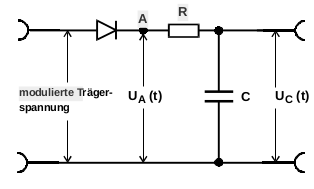
\includegraphics[width=0.6\textwidth]{figures/gleichrichterdiode.PNG}
  \caption{Schaltbild zur Demodulation eines amplitudenmodulierten Signals mit Hilfe einer Diode.\cite{sample}}
  \label{fig:8}
\end{figure}

\begin{figure}
\centering
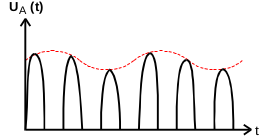
\includegraphics[width=0.6\textwidth]{figures/spannung_diode.PNG}
\caption{Spannungsverlauf nach Gleichrichten durch Diode.\cite{sample}}
\label{fig:gleichgerichtet}
\end{figure}

\FloatBarrier

\paragraph{Demodulationsschaltung für frequenzmodulierte Signale}
\mbox{}\\
Um ein frequenzmoduliertes Signal zu demodulieren, kann ein
\textit{Flankendemodulator} genutzt werden.
Eine schematische Darstellung eines solchen ist in Abbildung \ref{fig:11}
gegeben. Für die Demodulation wird der Schwingkreis so eingestellt, dass
die steile Flanke der Resonanzkurve, $\omega_{\text{T}}$ beinhaltet.
Da sich die Frequenz der modulierten Schwingung gemäß dem Modulationssignals
verändert, erzeugt der Schwingkreis eine amplitudenmodulierte Spannung
$U_{\text{C}}(\omega)$. Aus dieser kann dann wie zuvor beschrieben das
Modulationssignal gewonnen werden.

\begin{figure}
\centering
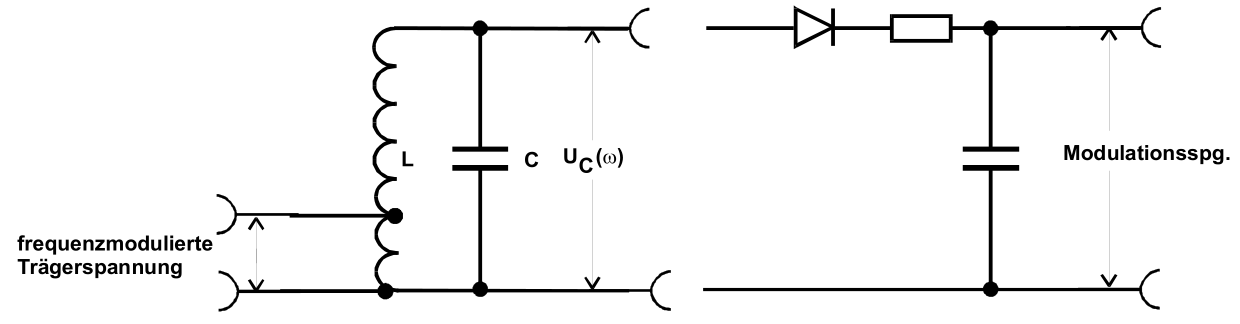
\includegraphics[width=0.7\textwidth]{figures/flankenmodulator.PNG}
\caption{Schaltbild eines Flankendemodulators.\cite{sample}}
\label{fig:11}
\end{figure}
